\begin{enumerate}[label=\alph*)]
    \item 
    ابتدا عکس وایرشارک را در این قسمت قرار می‌دهیم.
    \begin{center}
        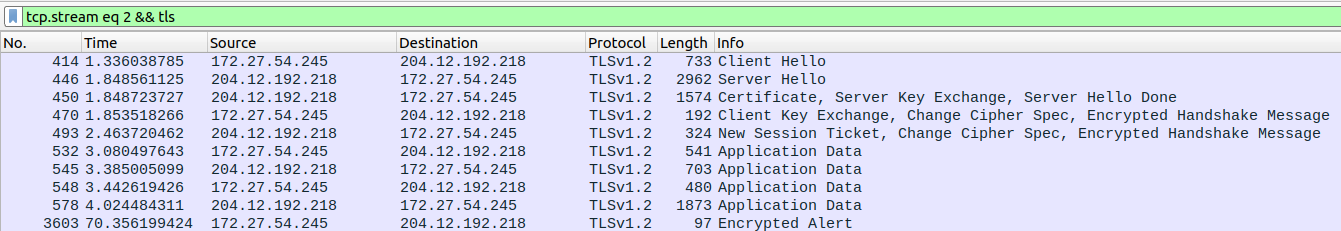
\includegraphics[scale=0.38]{pics/wireshark1.png}
    \end{center}
    فریم اول را کلاینت به سمت سرور ارسال کرده که عملا 
    \lr{Client Hello} 
    در \lr{tls handshake}
    است و پاسخ آنرا سرور با فریم دوم یعنی 
    \lr{Server Hello}
    داده است.
    سپس سرور و کلاینت در دو قسمت بعدی با یکدیگر تبادل کلید کرده‌اند و نهایتا 
    سرور یک 
    \lr{Session Ticket}
    ساخته و برای کلاینت ارسال می‌کند و بعد از ان صحبت کلاینت و سرور آغاز می‌شود.
    دیاگرام به صورت زیر است : 
    \begin{center}
        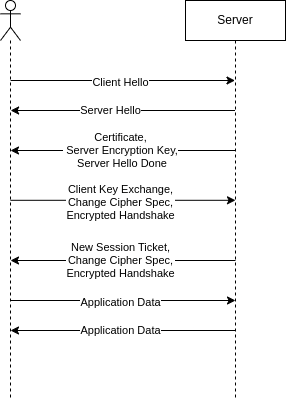
\includegraphics[scale=0.45]{pics/client.png}
    \end{center}
    حال طول فیلد‌ها را مشخص می‌کنیم.
    \begin{itemize}
        \item \lr{Client Hello} : 662 بایت
        \item \lr{Server Hello} : 76 بایت 
        \item \lr{Certificate} : 3971 بایت
        \item  \lr{Server Key Exchange} : 329 بایت
        \item \lr{Server Hello Done} : 4 بایت
        \item \lr{Client Key Exchange} : 70 بایت 
        \item \lr{Change Cipher Spec} : 1 بایت 
        \item \lr{Encrypted Handshake (Server)} : 40 بایت 
        \item \lr{New Session Ticket} : 202 بایت 
        \item \lr{Change Cipher Spec} : 1 بایت 
        \item \lr{Encrypted Hanshake} : 40 بایت
    \end{itemize}
    \begin{center}
        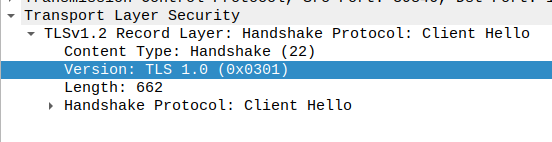
\includegraphics[scale=0.38]{pics/w1.png}
        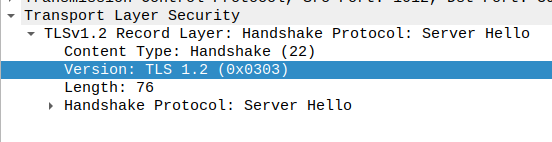
\includegraphics[scale=0.38]{pics/w2.png}
        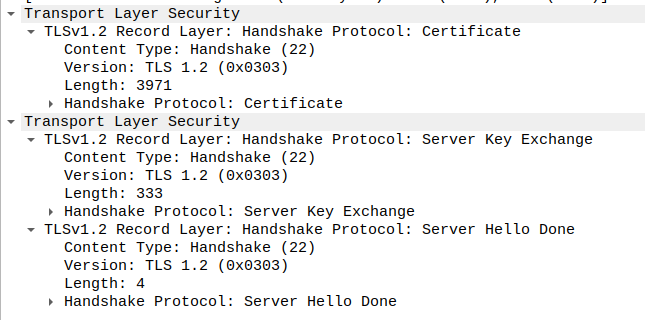
\includegraphics[scale=0.38]{pics/w3.png}
        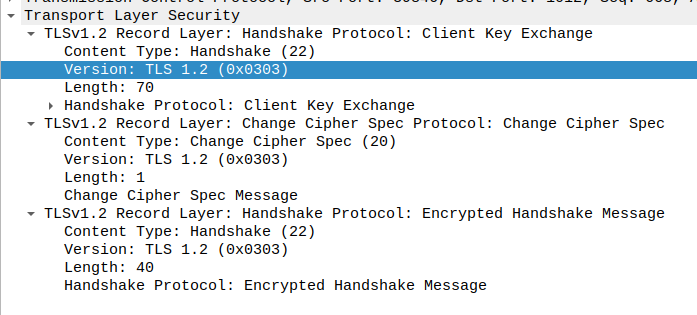
\includegraphics[scale=0.38]{pics/w4.png}
        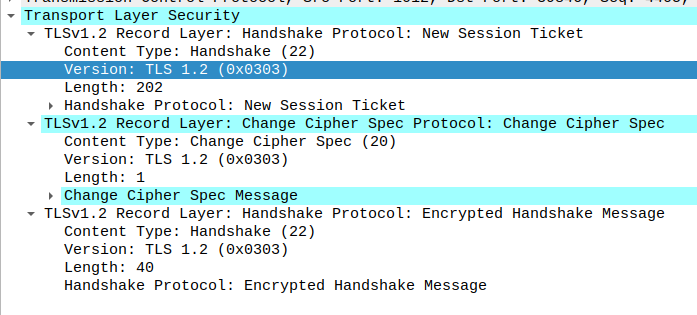
\includegraphics[scale=0.38]{pics/w5.png}
    \end{center}
    \item 
    \textbf{\lr{Client Hello}}
    \begin{itemize}
        \item \lr{Content Type} : Handshake
        \item \lr{Nonce (Challenge) } : اشاره به مقدار \textbf{random} دارد که عملا یک عدد رندوم \footnote{\lr{pseudo-random}} 
        ۳۲ بایتی دارد که برای این به کار می‌رود که سرور آن را عوض کرده
        و کلاینت مطمئن شود که حمله \lr{replay attack}
        رخ نداده است. همچنین در ابتدای هر session این عدد به صورت یکتا برای همان session ساخته می‌شود که 
        عملا در صورتی که حمله‌کننده به سشن‌های قبلی دست یابد نمی‌تواند آنها را بازارسال کند. همچنین از این رندوم برای ساخت \lr{Master Key} در قدم‌های بعدی استفاده می‌شود.
        \item \lr{Cipher Suites} : مجموعه‌ای از الگوریتم‌های رمزنگاری پشتیبانی شده. می‌توانید لیست آنها را در عکس زیر مشاهده کنید.
        \begin{center}
            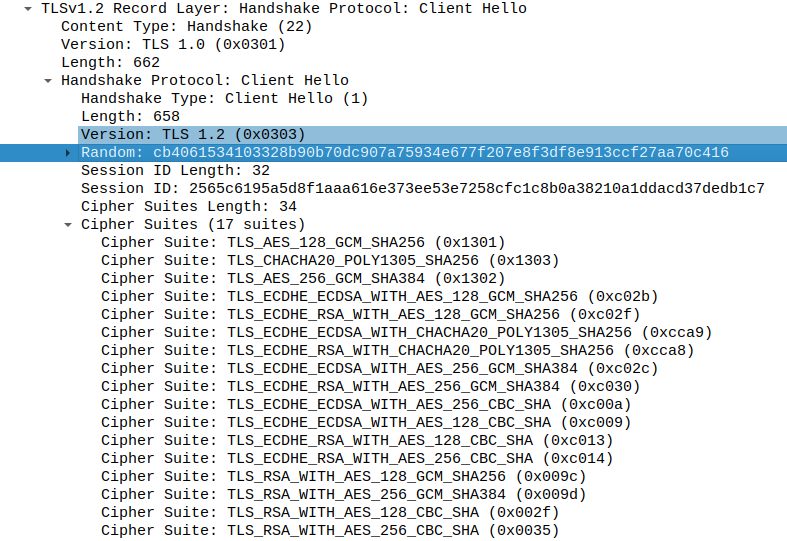
\includegraphics[scale=0.5]{pics/client_hello.png}
        \end{center}
    \end{itemize}
    \item 
    \textbf{\lr{Server Hello}}
    \begin{itemize}
        \item \lr{Cipher Suite} : \lr{TLS\_ECDHE\_RSA\_WITH\_AES\_256\_GCM\_SHA384 (0xc030)}
        \item Nounce : مانند \lr{Client Hello} یک Random که به آن \lr{Server Random} می‌گوییم ساخته می‌شود و به کلاینت ارسال می‌شود.
        \item \lr{Session ID} : یک مقدار یکتا است که برای resume کردن 
        سشن‌های قبلی به کار می‌رود و عملا باعث می‌شود که یک handshake کامل دیگر نیاز نباشد. در این کانکشن ما \lr{Session ID} نداشتیم 
        که به این معنی است که از قبل سشنی وجود نداشته و یا سرور \lr{Session Resume} را ساپورت نمی‌کند.
        \begin{center}
            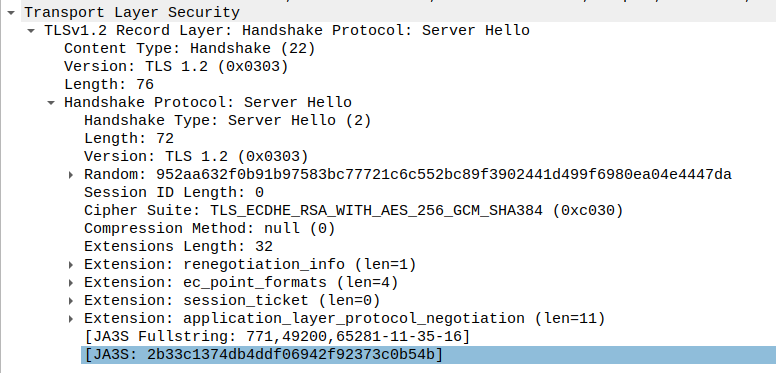
\includegraphics[scale=0.5]{pics/server_hello.png}
        \end{center}
        \item Certificate : در فریم دیگری ارسال شده که در قسمت بعدی آنرا توضیح می‌دهیم.
    \end{itemize}
    \item 
    \textbf{\lr{Certificate}}
    \begin{itemize}
        \item الگوریتم رمزنگاری کلید عمومی : \lr{RSAEncryption}
        \item طول کلید عمومی : از قسمت subjectPublicKey قابل محاسبه است که 2048 بیت است.
        \item الگوریتم امضا : \lr{sha256WithRSAEncryption}
        \item مقدار امضا : در پایین همان قسمت در encrypted 
        در عکس زیر می‌توانید آنرا به فرمت \lr{C Array} مشاهده کنید.
        \begin{center}
            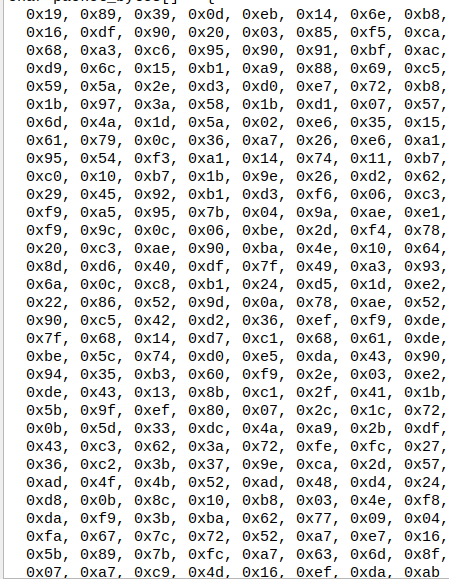
\includegraphics[scale=0.35]{pics/signiture.png}
        \end{center}
        \item صادرکننده گواهی : می‌توانید در عکس زیر صادرکننده گواهی را ببینید : 
        \begin{center}
            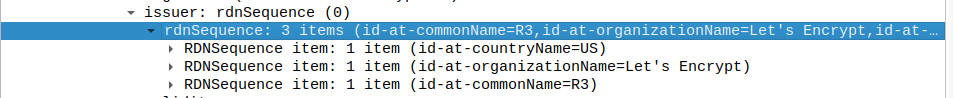
\includegraphics[scale=0.5]{pics/issuer.png}
        \end{center}
    \end{itemize}
    \item \textbf{\lr{Client Key Exchange}}
    \begin{itemize}
        \item \lr{Pre-Master Secret} : مقداری که به صورت مستقیم از تبادل کلید‌های عمومی بدست می‌آید. مثلا این مقدار در تبادل کلید 
        \lr{Diffie-Hellman} از این رابطه بدست می‌اید : $g^{ab} mod p$ در تبادل کلید به روش دیفی هلمن این مقدار عملا همان Pubkey ارسال شده است.
        در عکس زیر می‌توانید این Pubkey را مشاهده کنید. 
        \begin{center}
            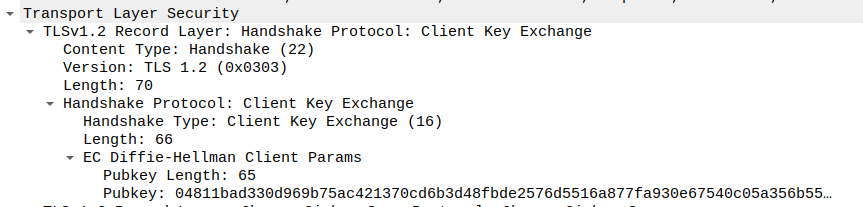
\includegraphics[scale=0.5]{pics/dh_key.png}
        \end{center}
    \end{itemize}
    \item \textbf{\lr{Change Cipher Spec}} : این پیام از طرف سرور و کلاینت برای یکدیگر ارسال می‌شود تا 
    مشخص کند که تمامی پیام‌های آینده به واسطه 
    \lr{Cipher Suite} 
    مشخص‌شده رمزنگاری می‌شوند. مقداری که سرور ارسال می‌کند با مقداری که کلاینت ارسال می‌کند یکسان نیست. دلیل این تفاوت این است که طرفی که پیام اولیه را ارسال کرده 
    مطمئن شود پیام دریافتی تازه و عملا بازارسال نشده است.
    \item \textbf{\lr{Application Data}} : پس از تبادل کلید و طی شدن مراحل handshake
    با الگوریتم رمزنگاری مشخص شده که در این مورد مثلا AES است رمزنگاری داده انجام شده و از آن به بعد ارتباط 
    کلاینت و سرور با آن و کلید مشترکشان رمزنگاری می‌شود.
\end{enumerate}